\chapter{赋范空间}
\label{chap:normed-spaces}
\label{chap:functional-analysis-and-approximation}

用$x^2$近似$[0,1]$上的$x$，误差有多大？若关心最坏的位置，可以取$\max_x\lvert x-x^2\rvert=\tfrac14$；若关心整体的累计偏差，可以取$\int_0^1\lvert x-x^2\rvert\,dx=\tfrac16$。两个数都合理，回答的是不同的问题。一列近似函数是否收敛，也要先说清用哪一种误差。上一章把函数当作向量，却还没有规定函数之间的距离；本章用范数做这件事，并研究不同范数下的收敛与极限。

第~\ref{sec:nspace-norms}节把卷二的范数公理用于整个函数，说明范数怎样给出收敛与柯西列，并借助上一章两两远离的单位列说明：无限维空间上总可以构造不等价的范数，同一列函数在一种范数下收敛、在另一种下可能不收敛。范数选定以后，还要问柯西列的极限是否仍在空间内，这是第~\ref{sec:nspace-banach-spaces}节的完备性。

随后三节给出具体的完备空间。第~\ref{sec:nspace-continuous-function-spaces}节证明紧集上的连续函数在最大误差下完备，而同一个集合在积分误差下不完备。为了给积分误差下的极限找到去处，第~\ref{sec:nspace-lp-spaces}节和第~\ref{sec:nspace-linfty-space}节在可测函数的几乎处处等价类上建立$L^p$与$L^\infty$，证明Hölder与Minkowski不等式和完备性。最后，第~\ref{sec:nspace-convergence-of-sequences}节比较逐点、一致、$L^p$及依测度收敛分别控制什么误差，并用一致可积性说明何时可以从依测度收敛得到积分收敛。

本章所用的测度与积分来自第~\ref{chap:measure}章和第~\ref{chap:integration}章，度量空间中的收敛、柯西列与完备性来自第~\ref{chap:metric-spaces}章，映射列的一致收敛来自第~\ref{chap:metric-space-maps}章。内积带来的正交结构在第~\ref{chap:inner-product-spaces}章研究；空间之间的包含映射作为有界算子在第~\ref{chap:linear-operators}章研究；简单函数、连续函数在$L^p$中的稠密性等逼近问题在第~\ref{chap:function-approximation}章研究。

\section{范数}
\label{sec:nspace-norms}

要判断两个函数整体上是否接近，先要给它们的差$f-g$规定一个“大小”，再用这个大小是否趋于零来判断近似是否成功。卷二已经用范数公理规定了向量的大小，本节把这套公理用到整个函数上。先说明函数范数的含义，再说明它给出的收敛与柯西列，最后说明无限维空间中不同范数之间可能无法互相控制。

\subsection{函数的范数}
\label{sec:nspace-function-norms}

函数的范数衡量的是整个函数的大小，而不是某一点处的函数值。要让不同的大小规则共享同一套推理，只要求它们满足几条共同的性质，这就是卷二的范数公理。

\begin{definition}[范数与赋范空间]
\label{def:nspace-norm}
设$V$是$\mathbb K$上的线性空间。映射$\lVert\cdot\rVert:V\to[0,\infty)$称为$V$上的\term{范数}（norm），若对所有$f,g\in V$与$c\in\mathbb K$：
\begin{enumerate}
 \item 正定性：$\lVert f\rVert=0$当且仅当$f=0$；
 \item 齐次性：$\lVert cf\rVert=\lvert c\rvert\,\lVert f\rVert$；
 \item 三角不等式：$\lVert f+g\rVert\leq\lVert f\rVert+\lVert g\rVert$。
\end{enumerate}
配备范数的线性空间$(V,\lVert\cdot\rVert)$称为\term{赋范空间}（normed space）。
\end{definition}

对函数而言，正定性中的“$f=0$”指$f$是零元素。在逐点运算的函数空间里，零元素是处处为零的函数，所以$\lVert f\rVert=0$必须迫使$f$在每一点都为零。齐次性说明把函数整体放大$c$倍，大小也放大$\lvert c\rvert$倍。三角不等式说明两段误差串联起来不超过各自之和，它是后面误差估计的基本工具。有限维范数的例子与性质，可参考\BookChapterRef{chap:normed-inner-product-spaces}{卷二第3章“赋范空间与内积空间”}。

\paragraph{两种整体大小}
在$C[0,1]$上，最常用的两种大小是
\[
 \lVert f\rVert_\infty=\max_{x\in[0,1]}\lvert f(x)\rvert,\qquad \lVert f\rVert_1=\int_0^1\lvert f(x)\rvert\,dx.
\]
前者看最坏的位置，后者看绝对值曲线下的总面积。对$h(x)=x-x^2$，$\lVert h\rVert_\infty=\tfrac14$，$\lVert h\rVert_1=\tfrac16$，这就是章首的两个数。两者都不是函数在某一点的值：$h(0)=0$，但$h$并不是零元素。

逐条核对公理。$\lVert\cdot\rVert_\infty$的齐次性和三角不等式在每个$x$处成立后取最大值即得；若最大值为$0$，则每点$\lvert f(x)\rvert=0$。$\lVert\cdot\rVert_1$的齐次性与三角不等式来自积分的线性与单调性。正定性需要连续：若$f$在某点$x_0$处$\lvert f(x_0)\rvert=a>0$，则在$x_0$附近的一个区间上$\lvert f\rvert>a/2$，积分为正。

\paragraph{有限性与正定性要逐个空间核验}
同一个公式放到别的函数集合上，公理可能不再成立。把$\int_0^1\lvert f\rvert$用于$[0,1]$上的有界黎曼可积函数，正定性失效：只在$x=\tfrac12$处取$1$、其余处取$0$的函数不是零函数，积分却为$0$。这样只满足齐次性与三角不等式、允许非零元素大小为零的函数称为\term{半范数}（seminorm）。

公式的值也可能是无穷。把$\max\lvert f\rvert$换成$\sup\lvert f\rvert$用于$\mathbb R$上的连续函数，$f(x)=x$的上确界为$+\infty$，不是实数。所以给一个函数集合配范数时，要分别核验三件事：集合对线性运算封闭，公式对集合中每个元素有限，正定性在这个集合上成立。第~\ref{sec:nspace-continuous-function-spaces}节到第~\ref{sec:nspace-linfty-space}节对各个具体空间逐一完成这些核验，其中积分范数的正定性要靠把几乎处处相等的函数看作同一个元素来恢复。

\subsection{范数与收敛}
\label{sec:nspace-norm-convergence}

范数给出距离$d(f,g)=\lVert f-g\rVert$。由三条公理可以直接验证距离公理，例如三角不等式$d(f,h)=\lVert(f-g)+(g-h)\rVert\leq d(f,g)+d(g,h)$。所以每个赋范空间都是度量空间，第~\ref{chap:metric-spaces}章关于点列收敛、柯西列、闭集和完备性的结论都可以直接使用。

\paragraph{依范数收敛与柯西列}
按这个距离，序列$(f_n)$收敛到$f$就是$\lVert f_n-f\rVert\to0$，称为\term{依范数收敛}（convergence in norm）。$(f_n)$是柯西列，就是对每个$\varepsilon>0$存在$N$，使$m,n\geq N$时$\lVert f_n-f_m\rVert<\varepsilon$。收敛列都是柯西列；反过来是否成立取决于空间，这是下一节的问题。

范数的选择决定了收敛控制什么。在$C[0,1]$上，$\lVert f_n-f\rVert_\infty\to0$说明对每个$\varepsilon>0$，从某个$N$起，所有输入处的误差同时不超过$\varepsilon$，这正是一致收敛。$\lVert f_n-f\rVert_1\to0$只说明误差曲线下的面积趋于零，允许在越来越窄的区间上保留较大的误差。由$\lVert h\rVert_1\leq\lVert h\rVert_\infty$，一致收敛推出积分误差收敛；下一小节将说明反过来不成立。

\paragraph{等价范数}
若同一空间上的两个范数能互相控制，它们给出的收敛判断就完全一致。

\begin{definition}[等价范数]
\label{def:nspace-equivalent-norms}
线性空间$V$上的两个范数$N_1,N_2$称为\term{等价范数}（equivalent norms），若存在常数$0<c\leq C$，使对所有$f\in V$，
\[
 c\,N_1(f)\leq N_2(f)\leq C\,N_1(f).
\]
\end{definition}

对$h=f_n-f$使用右边的不等式，$N_1(f_n-f)\to0$推出$N_2(f_n-f)\to0$；左边的不等式给出反方向。对$h=f_n-f_m$使用同样的不等式，两个范数下的柯西列也相同。所以等价范数给出相同的收敛序列、相同的极限和相同的柯西列，完备性也随之相同。关键是常数$c,C$与$f$无关。

有限维空间中，任意两个范数都等价，卷二已经证明了这一点。因此有限维空间的收敛与完备性不依赖范数的选择，只有误差的具体数值与常数随范数改变。卷二的证明用到有限维单位球面的紧性，上一章说明这一性质在无限维中失效，所以无限维空间中的两个范数是否等价，需要另作判断。

\subsection{范数不等价}
\label{sec:nspace-inequivalent-norms}

下面先从一般的无限维赋范空间出发，构造一个与原范数不等价的新范数，再在$C[0,1]$上给出一对具体的不等价范数。

\paragraph{用代数基构造}
设$(X,N_1)$是无限维赋范空间，$\{e_n\}_{n\geq1}$是第~\ref{chap:functions-as-vectors}章用Riesz引理构造的单位列：$N_1(e_n)=1$，且$\{e_n\}$线性无关。用选择公理可以把这个线性无关族扩充为$X$的一组代数基$B\supseteq\{e_n\}$，这里不给出证明。每个$x\in X$都唯一地写成$B$中有限个元素的组合。

在基上规定$Te_n=e_n/n$，对其余的$b\in B$规定$Tb=b$，再线性延拓：对$x=\sum_{b}c_bb$（有限和），令$Tx=\sum_bc_b\lambda_bb$，其中$\lambda_{e_n}=1/n$，其余$\lambda_b=1$。表示唯一，所以$T$是定义合理的线性映射。$T$还是单射：若$Tx=0$，由表示的唯一性，每个$c_b\lambda_b=0$，而$\lambda_b\neq0$，故每个$c_b=0$。

令$N_2(x)=N_1(Tx)$。它是范数：齐次性与三角不等式由$T$的线性和$N_1$的相应性质得到，例如$N_2(x+y)=N_1(Tx+Ty)\leq N_2(x)+N_2(y)$；若$N_2(x)=0$，则$Tx=0$，由单射得$x=0$。但
\[
 N_1(e_n)=1,\qquad N_2(e_n)=N_1(e_n/n)=\frac1n.
\]
若存在$c>0$使$cN_1\leq N_2$，取$x=e_n$得$c\leq1/n$对所有$n$成立，矛盾。所以$N_1$与$N_2$不等价：序列$e_n$在$N_2$下趋于零，在$N_1$下却始终与零相距$1$。

这个构造说明，每个无限维赋范空间上都存在与原范数不等价的范数。它是纯粹的存在性论证：代数基无法具体写出，$N_2$也就无法具体计算。

\paragraph{连续函数上的一对具体范数}
在$C[0,1]$上，$\lVert\cdot\rVert_\infty$与$\lVert\cdot\rVert_1$就不等价。一个方向的控制成立：$\lvert f(x)\rvert\leq\lVert f\rVert_\infty$对每个$x$成立，在$[0,1]$上积分得$\lVert f\rVert_1\leq\lVert f\rVert_\infty$。另一个方向没有常数：取$f_n(x)=x^n$，
\[
 \lVert x^n\rVert_\infty=1,\qquad \lVert x^n\rVert_1=\int_0^1x^n\,dx=\frac1{n+1}\to0.
\]
若$\lVert f\rVert_\infty\leq C\lVert f\rVert_1$，则$1\leq C/(n+1)$对所有$n$成立，矛盾。

图~\ref{fig:nspace-xn-norms}显示了这一差别的来源。$x^n$只在靠近$1$的越来越窄的区间上取较大的值，积分看到的是这段区间的面积，最大值看到的是峰顶。同一列函数在积分范数下趋于零函数，在最大值范数下与零函数的距离始终为$1$。图中的平方积分大小$\lVert x^n\rVert_2=(2n+1)^{-1/2}$在第~\ref{sec:nspace-lp-spaces}节正式定义。

\begin{figure}[!htb]
  \centering
  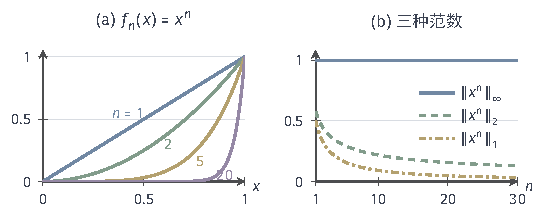
\includegraphics[width=92.3mm]{figures/02-abstract-mathematics/03-function-spaces/tikz/c1-xn-norms/figure.pdf}
  \caption{$x^n$在$[0,1]$上的三种大小。(a)$n=1,2,5,20$时的曲线，较大的函数值集中到右端越来越窄的区间上。(b)三种大小随$n$的变化：$\lVert x^n\rVert_\infty=1$保持不变，$\lVert x^n\rVert_2=(2n+1)^{-1/2}$与$\lVert x^n\rVert_1=(n+1)^{-1}$趋于零。}
  \label{fig:nspace-xn-norms}
\end{figure}

\paragraph{与有限维的对照}
卷二的结论是“有限维空间中任意两个范数都等价”。它在无限维中的否定是“存在不等价的范数”，而不是“任意两个范数都不等价”。例如$\lVert\cdot\rVert_\infty$与$2\lVert\cdot\rVert_\infty$在任何空间上都等价，常数为$c=C=2$。

因此在无限维空间中谈论收敛，必须同时说明用哪个范数。说“$x^n$在$C[0,1]$中收敛到$0$”是不完整的陈述：在$\lVert\cdot\rVert_1$下它成立，在$\lVert\cdot\rVert_\infty$下它不成立。后面各节始终把空间与范数一起给出。

\section{Banach空间}
\label{sec:nspace-banach-spaces}

迭代算法、级数截断和逐步加细的逼近，常常只告诉我们近似之间越来越接近，即得到一个柯西列，而不直接给出极限。要从“彼此接近”推出“存在极限”，空间里必须真有这个极限。范数规定了怎样衡量接近，却不保证这一点；后者是空间与范数共同的性质。

\begin{definition}[Banach空间]
\label{def:nspace-banach}
若赋范空间$V$中的每个柯西列都依范数收敛到$V$中的某个元素，即范数诱导的度量空间是完备的，称$V$是\term{完备}（complete）的赋范空间，也称\term{Banach空间}（Banach space）。
\end{definition}

这就是第~\ref{chap:metric-spaces}章的完备性，只是度量来自范数。卷二已经证明有限维赋范空间在任意范数下都完备，所以有限维时无需另作核验。无限维时，完备与否要逐个空间证明；同一个集合换一个范数，结论可能改变，第~\ref{sec:nspace-continuous-function-spaces}节会给出这样的例子。

\paragraph{闭子空间判据}
很多函数空间是另一个已知完备空间的子空间。这时可以借用第~\ref{chap:metric-spaces}章的两个结论：完备度量空间中的闭子集是完备的；任何度量空间中的完备子集都是闭集。用在Banach空间$X$的线性子空间$M$上，就得到下面的判据。

\begin{theorem}[闭子空间判据]
\label{thm:nspace-closed-subspace}
设$X$是Banach空间，$M\subseteq X$是线性子空间，$M$带有限制后的范数。则$M$是Banach空间当且仅当$M$是$X$中的闭集。
\end{theorem}

\begin{proof}
设$M$闭，$(f_n)$是$M$中的柯西列。它也是$X$中的柯西列，由$X$完备收敛到某个$f\in X$；$M$闭，所以$f\in M$。反过来，设$M$完备，$f_n\in M$且在$X$中$f_n\to f$。收敛列是柯西列，所以$(f_n)$是$M$中的柯西列，在$M$中收敛到某个$g$；$X$中极限唯一，$f=g\in M$，所以$M$闭。
\end{proof}

两个方向的分工不同。从闭推出完备时，大空间$X$的完备性提供极限，$M$的闭性保证极限没有离开$M$。从完备推出闭时，并不需要$X$完备，第~\ref{chap:functions-as-vectors}章证明有限维子空间闭性时用的正是这一方向。

\paragraph{不闭的子空间}
多项式给出一个不完备的例子。在$[0,1]$上用$\lVert f\rVert_\infty=\max_x\lvert f(x)\rvert$衡量多项式，取$e^x$的Taylor多项式$p_N(x)=\sum_{k=0}^Nx^k/k!$。由Lagrange余项，
\[
 \max_{x\in[0,1]}\lvert e^x-p_N(x)\rvert\leq\frac{e}{(N+1)!}\to0,
\]
所以对$m>n$，$\lVert p_m-p_n\rVert_\infty\leq\frac{e}{(m+1)!}+\frac{e}{(n+1)!}$，$(p_N)$是多项式空间中的柯西列。

它在多项式空间中没有极限。若有多项式$p$使$\lVert p_N-p\rVert_\infty\to0$，则对每个$x$都有$p_N(x)\to p(x)$；又$p_N(x)\to e^x$，所以$p=e^x$在$[0,1]$上成立。但多项式求足够多次导数后恒为零，$e^x$的各阶导数都不为零，矛盾。所以多项式空间在最大误差下不完备；下一节证明$C[0,1]$完备后，闭子空间判据说明这等价于多项式空间在$C[0,1]$中不闭。

\paragraph{范数与完备性是两个问题}
给一个函数集合配范数，回答的是“怎样衡量误差”；问它是否完备，回答的是“误差趋零的过程能否在集合内找到终点”。前者只要核验三条公理，后者要分析柯西列的极限。不完备的赋范空间仍然是合法的赋范空间，只是不能仅凭柯西性断言极限存在。

不完备的空间可以通过补入极限变成完备的：第~\ref{chap:metric-spaces}章的完备化构造对赋范空间同样适用，线性运算和范数都可以沿柯西列延拓。但抽象完备化只保证新元素存在，不说明它们是哪一类函数。本章采用另一条路：直接在更大的函数集合上定义范数，再证明这个具体的空间完备，第~\ref{sec:nspace-lp-spaces}节的$L^p$就是这样得到的。

\section{连续函数空间}
\label{sec:nspace-continuous-function-spaces}

连续函数是最接近一元分析经验的函数空间。本节先在紧度量空间上配以最大绝对值范数，证明它是Banach空间；再看定义域不紧时需要怎样调整；最后把同一个$C[0,1]$换成积分范数，看完备性怎样失去。

\paragraph{紧集上的一致范数}
设$K$是非空紧度量空间，$C(K)$为$K$上的全体$\mathbb K$值连续函数，在逐点运算下它是线性空间。定义
\begin{equation}
 \lVert f\rVert_\infty=\max_{x\in K}\lvert f(x)\rvert .
 \label{eq:nspace-uniform-norm}
\end{equation}
$\lvert f\rvert$是紧集上的实值连续函数，由第~\ref{chap:topological-spaces}章“紧集的连续像是紧集”，它的值域是$\mathbb R$中的紧集，所以最大值存在且有限。

这个范数称为\term{一致范数}（uniform norm），也称上确界范数。它的公理核验与上一节对$C[0,1]$的论证相同：在每个$x$处验证，再取最大值。当$K=\{1,\ldots,d\}$是有限集时，$C(K)$就是$\mathbb K^d$配最大分量范数，这正是函数作为向量的类比中最贴切的一个情形。

\paragraph{一致范数下的收敛}
$\lVert f_n-f\rVert_\infty\leq\varepsilon$意味着在所有$x\in K$处同时有$\lvert f_n(x)-f(x)\rvert\leq\varepsilon$，即$f_n$的整条曲线落在以$f$为中心、上下宽$\varepsilon$的带子里。所以一致范数下的收敛就是第~\ref{chap:metric-space-maps}章的一致收敛。

图~\ref{fig:nspace-uniform-tube}(a)是一个落在带内的例子。图~\ref{fig:nspace-uniform-tube}(b)中的$x^n$在$[0,1)$上逐点趋于$0$，但每条曲线都会在靠近$1$处越出零函数周围的带子，越出点随$n$右移却始终存在。

\begin{BookInlineFigure}
  \centering
  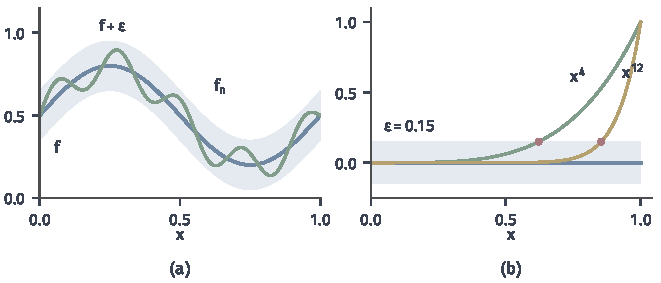
\includegraphics[width=112mm]{figures/04-spaces-measures-and-geometry/03-function-spaces/matplotlib/nspace-uniform-tube/figure.pdf}
  \caption{一致范数的几何意义，浅蓝色为半宽$\varepsilon=0.15$的带子。(a)$f(x)=0.5+0.3\sin(2\pi x)$（蓝）周围的带子，$f_n=f+0.1\sin(9\pi x)$（绿）整条曲线都在带内，所以$\lVert f_n-f\rVert_\infty=0.1$。(b)零函数周围的带子；$x^4$与$x^{12}$分别在红点$x=0.15^{1/4}$和$x=0.15^{1/12}$处越出带子。}
  \label{fig:nspace-uniform-tube}
\end{BookInlineFigure}

$x^n$在这个范数下连柯西列都不是。令$t=x^n$，当$x$跑遍$[0,1]$时$t$也跑遍$[0,1]$，所以
\[
 \lVert x^n-x^{2n}\rVert_\infty=\max_{t\in[0,1]}(t-t^2)=\frac14,
\]
这个值不随$n$减小。

\paragraph{完备性}
第~\ref{chap:metric-space-maps}章已经为一致收敛建立了两个结论：目标空间完备时，一致柯西的映射列一致收敛到某个映射；连续映射列的一致极限仍连续。$\mathbb K$是完备的，把两者合起来，就得到连续函数空间的完备性。

\begin{theorem}[紧集上连续函数空间的完备性]
\label{thm:nspace-ck-complete}
设$K$是非空紧度量空间。则$(C(K),\lVert\cdot\rVert_\infty)$是Banach空间。
\end{theorem}

\begin{proof}
设$(f_n)$是$C(K)$中的柯西列。对每个$\varepsilon>0$，存在$N$，使$m,n\geq N$时
\[
 \max_{x\in K}\lvert f_n(x)-f_m(x)\rvert<\varepsilon,
\]
这正说明$(f_n)$作为映射列是一致柯西的。

$\mathbb K$完备，所以$f_n$一致收敛到某个函数$f:K\to\mathbb K$。各$f_n$连续，一致极限$f$也连续，于是$f\in C(K)$。一致收敛就是$\lVert f_n-f\rVert_\infty\to0$，所以柯西列在$C(K)$中收敛。
\end{proof}

证明中三件事各有出处：候选极限由$\mathbb K$的完备性逐点给出；共同的误差阈值把逐点收敛加强为一致收敛；一致收敛保证极限连续。$K$的紧性只用来保证最大值有限，使式~\eqref{eq:nspace-uniform-norm}是范数。

\paragraph{非紧定义域}
在非紧的度量空间$X$上，连续函数可能无界，例如$\mathbb R$上的$f(x)=x$，一致“范数”不再是实数。这时只保留有界的连续函数，并把最大值换成上确界：
\begin{equation}
 C_b(X)=\Bigl\{f:X\to\mathbb K\ \text{连续}:\ \sup_{x\in X}\lvert f(x)\rvert<\infty\Bigr\},
 \label{eq:nspace-cb}
\end{equation}
范数为
\[
 \lVert f\rVert_\infty=\sup_{x\in X}\lvert f(x)\rvert.
\]
有界函数之和与数乘仍有界，所以$C_b(X)$是线性空间。

定理~\ref{thm:nspace-ck-complete}的证明中，候选极限的存在和连续都没有用到紧性。非紧时只需补充一步：一致极限仍然有界。取$N$使$n\geq N$时$\sup_x\lvert f_n(x)-f(x)\rvert\leq1$，则对每个$x$，
\[
 \lvert f(x)\rvert\leq\lvert f_N(x)\rvert+1\leq\lVert f_N\rVert_\infty+1,
\]
右边与$x$无关。于是$f\in C_b(X)$，所以$(C_b(X),\lVert\cdot\rVert_\infty)$对任意度量空间$X$都是Banach空间。

非紧定义域上会出现紧区间上没有的现象。在$C_b(\mathbb R)$中取移动的三角形
\[
 f_n(x)=\max\bigl(0,\ 1-\lvert x-n\rvert\bigr).
\]
每个固定的$x$在$n>\lvert x\rvert+1$以后都有$f_n(x)=0$，所以$f_n$逐点趋于零；但峰高始终为$1$，$\lVert f_n\rVert_\infty=1$，序列不依范数收敛。质量没有消失，只是移向无穷远，这与向量的单位列$e_n$的情形相同。

\paragraph{积分范数下的不完备}
回到$C[0,1]$，改用积分范数$\lVert f\rVert_1=\int_0^1\lvert f(x)\rvert\,dx$，其中积分对Lebesgue测度取，连续函数的Lebesgue积分与黎曼积分相同。集合没有变，只换了衡量误差的方式，完备性却会失去。

对$n\geq2$，令
\[
 g_n(x)=\begin{cases}0,&0\leq x\leq\frac12,\\ n\bigl(x-\frac12\bigr),&\frac12<x<\frac12+\frac1n,\\ 1,&\frac12+\frac1n\leq x\leq1.\end{cases}
\]
每个$g_n$连续，越来越陡地从$0$升到$1$，像是在逼近$\tfrac12$处跳跃的阶跃函数$\mathbf 1_{(1/2,1]}$，如图~\ref{fig:nspace-step-ramp}(a)所示。

\begin{BookInlineFigure}
  \centering
  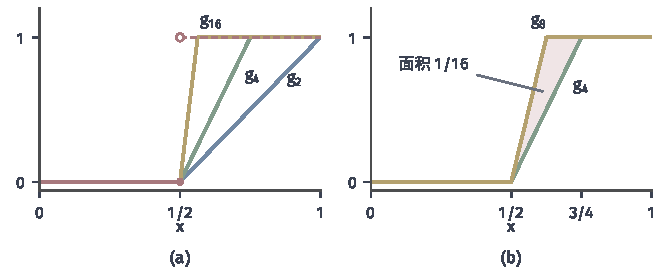
\includegraphics[width=112mm]{figures/04-spaces-measures-and-geometry/03-function-spaces/matplotlib/nspace-step-ramp/figure.pdf}
  \caption{积分范数下的柯西列。(a)折线$g_2,g_4,g_{16}$（蓝、绿、黄）越来越陡，红线是它们的积分极限$\mathbf 1_{(1/2,1]}$，空心圈表示跳跃。(b)$g_4$与$g_8$之间的浅红区域面积为$\lVert g_4-g_8\rVert_1=\tfrac1{16}$。}
  \label{fig:nspace-step-ramp}
\end{BookInlineFigure}

先算这列函数彼此的距离。设$m>n\geq2$，则$g_m\geq g_n$处处成立，所以
\[
 \lVert g_n-g_m\rVert_1=\int_0^1g_m\,dx-\int_0^1g_n\,dx.
\]
$g_n$下方的面积由一个底$\tfrac1n$、高$1$的三角形和宽$\tfrac12-\tfrac1n$的矩形组成，于是
\[
 \int_0^1g_n\,dx=\frac12-\frac1{2n}.
\]
代回前式，得到
\begin{equation}
 \lVert g_n-g_m\rVert_1=\frac1{2n}-\frac1{2m}.
 \label{eq:nspace-ramp-distance}
\end{equation}
例如$n=4$、$m=8$时距离是$\tfrac18-\tfrac1{16}=\tfrac1{16}$，就是图~\ref{fig:nspace-step-ramp}(b)中的面积。式~\eqref{eq:nspace-ramp-distance}小于$\tfrac1{2n}$，随$n$增大趋于零，所以$(g_n)$是柯西列。

下面证明它在$C[0,1]$中没有极限。假设存在$g\in C[0,1]$使$\lVert g_n-g\rVert_1\to0$。每个$g_n$在$[0,\tfrac12]$上为零，所以
\[
 \int_0^{1/2}\lvert g(x)\rvert\,dx\leq\int_0^1\lvert g_n(x)-g(x)\rvert\,dx\to0.
\]
左边不依赖$n$，只能为零；$\lvert g\rvert$连续且非负，故$g=0$在$[0,\tfrac12]$上处处成立。

再任取$\delta\in(0,\tfrac12)$。当$n>1/\delta$时，$g_n$在$[\tfrac12+\delta,1]$上恒为$1$，同样的论证给出
\[
 \int_{1/2+\delta}^1\lvert1-g(x)\rvert\,dx=0,
\]
所以$g=1$在$[\tfrac12+\delta,1]$上成立。$\delta$任意，所以$g$在$(\tfrac12,1]$上恒为$1$。于是$g(\tfrac12)=0$，而右侧极限为$1$，$g$在$\tfrac12$处不连续，矛盾。

所以$(C[0,1],\lVert\cdot\rVert_1)$不是Banach空间。同一列函数在一致范数下连柯西列都不是：取$x=\tfrac12+\tfrac1{2n}$，
\[
 \lvert g_{2n}(x)-g_n(x)\rvert=1-\frac12=\frac12.
\]

积分误差所指向的“极限”是阶跃函数，它不在连续函数之中，而且它在$\tfrac12$处取什么值并不影响积分。要让这样的极限有处可去，下一节把成员扩大为可测函数，并把几乎处处相等的函数看作同一个元素。

\section{\texorpdfstring{$L^p$}{Lp}空间}
\label{sec:nspace-lp-spaces}

上一节的折线列在积分误差下彼此越来越近，极限却是一个阶跃函数，不在连续函数之中。本节允许一般的可测函数，按$p$次幂累计偏差，并把在零测集上改动的函数看作同一个元素。这样得到的$L^p$空间满足范数公理，而且完备。

本节固定测度空间$(X,\mathcal A,\mu)$。可测函数、积分、单调收敛定理与Fatou引理见第~\ref{chap:measure}章和第~\ref{chap:integration}章。函数取值于$\mathbb K$，所有估计都只用到绝对值，实、复两种情形的论证相同。

\paragraph{几乎处处相等的函数}
在$[0,1]$上取Lebesgue测度，令$f\equiv0$，而$g$只在$x=\tfrac12$处取$1$、其余处取$0$。单点集的测度为零，所以$\int_0^1\lvert f-g\rvert\,dx=0$。用积分衡量误差时，这两个函数无法区分；若坚持把它们当作不同的元素，积分就只是半范数，正定性失效。

解决办法是把它们看作同一个元素。对两个可测函数，规定
\begin{equation}
 f\sim_\mu g\quad\Longleftrightarrow\quad \mu(\{x:f(x)\neq g(x)\})=0,
 \label{eq:nspace-ae-equivalence}
\end{equation}
即$f=g$在$\mu$下\term{几乎处处}（almost everywhere）成立。这是等价关系：自反与对称直接成立；若$f\sim_\mu g$且$g\sim_\mu h$，则
\[
 \{f\neq h\}\subseteq\{f\neq g\}\cup\{g\neq h\},
\]
两个零测集之并仍是零测集。与$f$几乎处处相等的可测函数全体记为$[f]$，称为$f$的\term{等价类}（equivalence class），$f$是它的一个代表。

等价类之间的运算借助代表定义：$[f]+[g]=[f+g]$，$c[f]=[cf]$。结果不依赖代表的选择：若$f'\sim_\mu f$、$g'\sim_\mu g$，则
\[
 \{f'+g'\neq f+g\}\subseteq\{f'\neq f\}\cup\{g'\neq g\}
\]
是零测集。所以可测函数的等价类组成线性空间，零元素是几乎处处为零的函数这一整类。

把函数看作向量时，这一步相当于放弃了“读取单个分量”。在Lebesgue测度下每个单点都是零测集，同一类中的代表可以在任意给定点取任意值，“$[f]$在$x_0$处的值”没有意义。若$\mu(\{x_0\})>0$，同一类的代表在$x_0$处必须取同一个值。点值读取何时有意义，是第~\ref{chap:linear-functionals}章和第~\ref{chap:rkhs}章的问题。

\paragraph{\texorpdfstring{$L^p$}{Lp}范数}
有了等价类，就可以用$p$次幂的积分衡量函数的大小。这相当于把向量的$p$范数$(\sum_i\lvert v_i\rvert^p)^{1/p}$中的求和换成积分。

\begin{definition}[$L^p$空间]
\label{def:nspace-lp}
设$1\leq p<\infty$。若可测函数$f$满足$\int_X\lvert f\rvert^p\,d\mu<\infty$，称$f$是$p$次可积的。$p$次可积函数的几乎处处等价类全体记为$L^p(\mu)$，并令
\begin{equation}
 \lVert f\rVert_p=\Bigl(\int_X\lvert f\rvert^p\,d\mu\Bigr)^{1/p}.
 \label{eq:nspace-lp-norm}
\end{equation}
当$X$是欧氏空间的可测子集$\Omega$、$\mu$为Lebesgue测度时，记为$L^p(\Omega)$。
\end{definition}

这里用代表$f$代写等价类$[f]$。定义需要核验三件事。其一，数值不依赖代表：若$f\sim_\mu g$，则$\lvert f\rvert^p$与$\lvert g\rvert^p$几乎处处相等，零测集上的改动不影响积分。其二，正定性：$\int\lvert f\rvert^p\,d\mu=0$当且仅当$\lvert f\rvert^p=0$几乎处处，即$[f]$是零元素，这正是引入等价类要换取的结果。齐次性直接由积分的线性得到。

其三，$L^p(\mu)$对加法封闭。$p\geq1$时函数$t\mapsto t^p$在$[0,\infty)$上凸，所以对$a,b\geq0$有
\[
 \Bigl(\frac{a+b}2\Bigr)^p\leq\frac{a^p+b^p}2,
\]
也就是$(a+b)^p\leq2^{p-1}(a^p+b^p)$。取$a=\lvert f(x)\rvert$、$b=\lvert g(x)\rvert$，由$\lvert f+g\rvert\leq a+b$积分得
\[
 \int_X\lvert f+g\rvert^p\,d\mu\leq2^{p-1}\Bigl(\int_X\lvert f\rvert^p\,d\mu+\int_X\lvert g\rvert^p\,d\mu\Bigr)<\infty.
\]
数乘只把积分乘以常数$\lvert c\rvert^p$，封闭性同样成立，所以$L^p(\mu)$是线性空间。剩下的三角不等式不能由这个粗略估计得到，要用下面的Hölder不等式。

\paragraph{不同的\texorpdfstring{$p$}{p}}
$p$越大，局部的大偏差在总量中所占的比重越大。比较$[0,1]$上的两个误差：$h_1\equiv1$处处偏差为$1$，$h_2=4\cdot\mathbf 1_{[0,1/4]}$只在四分之一的区间上偏差为$4$。按绝对值累计，两者一样大：
\[
 \lVert h_1\rVert_1=1,\qquad \lVert h_2\rVert_1=4\times\frac14=1.
\]
按平方累计，分散的误差仍是$1$，集中的误差翻了一倍：
\[
 \lVert h_1\rVert_2=1,\qquad \lVert h_2\rVert_2=\Bigl(16\times\frac14\Bigr)^{1/2}=2.
\]

一般地，同样的计算给出
\[
 \lVert h_2\rVert_p=\Bigl(4^p\cdot\frac14\Bigr)^{1/p}=4^{1-1/p},
\]
它随$p$增大而增大，趋于最大偏差$4$，见图~\ref{fig:nspace-lp-weight}。选择$p$就是选择怎样为大偏差计价。

\begin{BookInlineFigure}
  \centering
  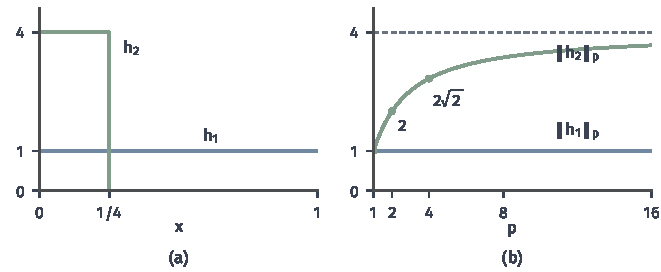
\includegraphics[width=112mm]{figures/04-spaces-measures-and-geometry/03-function-spaces/matplotlib/nspace-lp-weight/figure.pdf}
  \caption{$L^p$范数对大偏差的计价。(a)$[0,1]$上的两个误差：蓝色的$h_1\equiv1$与绿色的$h_2=4\cdot\mathbf 1_{[0,1/4]}$，二者$L^1$范数都是$1$。(b)$\lVert h_1\rVert_p\equiv1$，而$\lVert h_2\rVert_p=4^{1-1/p}$，在$p=1,2,4$处依次为$1,2,2\sqrt2$，虚线是$p\to\infty$时的极限$4$。}
  \label{fig:nspace-lp-weight}
\end{BookInlineFigure}

可积性也随$p$改变。在$(0,1]$上，$x^{-1/2}$属于$L^1$，因为
\[
 \int_0^1x^{-1/2}\,dx=2.
\]
它不属于$L^2$，因为$\int_0^1x^{-1}\,dx=\infty$。$x^{-1/4}$属于$L^2$，平方积分为$2$，但它在$0$附近无界。

\paragraph{数列空间}
取$X=\mathbb N_+$与\term{计数测度}（counting measure），即每个点的测度为$1$。可测函数就是数列$x=(x_k)$，积分就是求和，只有空集零测，等价类就是数列本身。$L^p$成为
\begin{equation}
 \ell^p=\Bigl\{x:\ \sum_{k\geq1}\lvert x_k\rvert^p<\infty\Bigr\},\quad \lVert x\rVert_p=\Bigl(\sum_{k\geq1}\lvert x_k\rvert^p\Bigr)^{1/p}.
 \label{eq:nspace-ellp}
\end{equation}
这是函数作为无限维向量最直接的情形：有限维向量可以看作后面全为零的数列，$\lVert x\rVert_p$就是卷二的坐标$p$范数的延伸。数列$x_k=1/k$属于$\ell^2$，因为$\sum_k1/k^2$收敛；它不属于$\ell^1$，因为调和级数发散。

\paragraph{Hölder与Minkowski不等式}
三角不等式的证明，关键在于控制乘积的积分。设$1<p<\infty$，取$q$满足$\tfrac1p+\tfrac1q=1$，即$q=p/(p-1)$，称$p,q$为\term{共轭指数}（conjugate exponents）。例如$p=2$时$q=2$，$p=3$时$q=\tfrac32$。

在有限维中，向量分量乘积之和有基本估计
\[
 \Bigl\lvert\sum_iu_iv_i\Bigr\rvert\leq\lVert u\rVert_p\lVert v\rVert_q,
\]
$p=q=2$时就是Cauchy--Schwarz不等式。下面把它搬到积分上，先从两个数的乘积开始。

\begin{lemma}[Young不等式]
\label{lem:nspace-young}
设$1<p<\infty$，$q$为其共轭指数。对任意$a,b\geq0$，
\begin{equation}
 ab\leq\frac{a^p}{p}+\frac{b^q}{q},
 \label{eq:nspace-young}
\end{equation}
等号当且仅当$a^p=b^q$。
\end{lemma}

\begin{proof}
固定$b\geq0$，考察$s\geq0$上的函数
\[
 F(s)=\frac{s^p}{p}-bs.
\]
求导得$F'(s)=s^{p-1}-b$，它在$s_*=b^{1/(p-1)}$处为零，在$s<s_*$时为负、$s>s_*$时为正，所以$F$在$s_*$处取唯一的最小值。

由$p/(p-1)=q$得$s_*^p=b^q$，又$bs_*=b^{1+1/(p-1)}=b^q$。代入$F$，于是
\[
 F(s_*)=\frac{b^q}{p}-b^q=-\frac{b^q}{q}.
\]
所以$F(a)\geq-b^q/q$，移项即得不等式；等号当且仅当$a=s_*$，即$a^p=b^q$。
\end{proof}

这个不等式有一幅面积图像。共轭条件等价于$(p-1)(q-1)=1$，所以曲线$s=t^{p-1}$也可以写成$t=s^{q-1}$。如图~\ref{fig:nspace-young-area}所示，曲线下方从$0$到$a$的面积是$a^p/p$，曲线左方从$0$到$b$的面积是$b^q/q$，两块区域合起来盖住矩形$[0,a]\times[0,b]$，所以面积之和不小于$ab$。

\begin{BookInlineFigure}
  \centering
  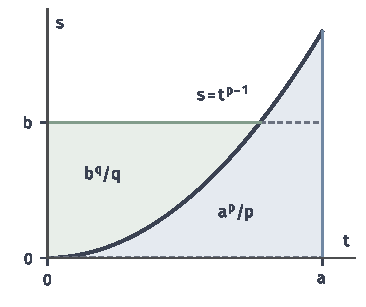
\includegraphics[width=62mm]{figures/04-spaces-measures-and-geometry/03-function-spaces/matplotlib/nspace-young-area/figure.pdf}
  \caption{Young不等式的面积解释，取$p=3$、$q=\tfrac32$、$a=1$、$b=0.6$。曲线为$s=t^2$，蓝色区域面积$a^p/p=\tfrac13$，绿色区域面积$b^q/q\approx0.310$，二者盖住虚线所示面积为$ab=0.6$的矩形。只有曲线恰好穿过矩形右上角，即$b=a^{p-1}$时，两块区域才恰好拼成矩形。}
  \label{fig:nspace-young-area}
\end{BookInlineFigure}

用图中的数字验算：$ab=0.6$，而$\tfrac13+0.310=0.643$，不等式成立且是严格的。若把$b$取成$a^{p-1}=1$，则$ab=1=\tfrac13+\tfrac23$，等号成立。

\begin{theorem}[Hölder不等式]
\label{thm:nspace-holder}
设$1<p<\infty$，$q$为其共轭指数，$f,g$是$X$上的可测函数。则
\begin{equation}
 \int_X\lvert fg\rvert\,d\mu\leq\lVert f\rVert_p\,\lVert g\rVert_q ,
 \label{eq:nspace-holder}
\end{equation}
其中右边允许取$+\infty$。特别地，$f\in L^p(\mu)$、$g\in L^q(\mu)$时$fg\in L^1(\mu)$。
\end{theorem}

\begin{proof}
若右边为$+\infty$，无需证明。若$\lVert f\rVert_p=0$，则$f=0$几乎处处，$fg=0$几乎处处，左边为零；$\lVert g\rVert_q=0$同理。下设$0<\lVert f\rVert_p,\lVert g\rVert_q<\infty$。

在Young不等式中逐点取$a=\lvert f(x)\rvert/\lVert f\rVert_p$、$b=\lvert g(x)\rvert/\lVert g\rVert_q$，得到
\[
 \frac{\lvert f(x)g(x)\rvert}{\lVert f\rVert_p\lVert g\rVert_q}\leq\frac{\lvert f(x)\rvert^p}{p\lVert f\rVert_p^p}+\frac{\lvert g(x)\rvert^q}{q\lVert g\rVert_q^q}.
\]
两边积分，右边等于$\tfrac1p+\tfrac1q=1$，再乘以$\lVert f\rVert_p\lVert g\rVert_q$即得结论。
\end{proof}

归一化的作用是把两个任意大小的函数缩放到“单位大小”，使右边两项积分后恰好凑成$1$。在$[0,1]$上取$f=x$、$g=x^2$、$p=3$、$q=\tfrac32$，此时$\lvert f\rvert^3=x^3=\lvert g\rvert^{3/2}$，两边相等：
\[
 \int_0^1x^3\,dx=\frac14,\qquad \Bigl(\frac14\Bigr)^{1/3}\Bigl(\frac14\Bigr)^{2/3}=\frac14,
\]
这与Young不等式的等号条件$a^p=b^q$相符。若取$f=1$、$g=x$、$p=q=2$，左边为$\tfrac12$，右边为$(\tfrac13)^{1/2}\approx0.577$，不等式是严格的。

\begin{theorem}[Minkowski不等式]
\label{thm:nspace-minkowski}
设$1\leq p<\infty$，$f,g\in L^p(\mu)$。则
\begin{equation}
 \lVert f+g\rVert_p\leq\lVert f\rVert_p+\lVert g\rVert_p.
 \label{eq:nspace-minkowski}
\end{equation}
因此$(L^p(\mu),\lVert\cdot\rVert_p)$是赋范空间。
\end{theorem}

\begin{proof}
$p=1$时，对逐点不等式$\lvert f+g\rvert\leq\lvert f\rvert+\lvert g\rvert$积分即可。

设$1<p<\infty$，记$I=\int\lvert f+g\rvert^p\,d\mu$。由封闭性的估计，$I<\infty$；若$I=0$，结论平凡，下设$I>0$。先把$p$次幂拆成两项：
\[
 \lvert f+g\rvert^p\leq\lvert f+g\rvert^{p-1}\lvert f\rvert+\lvert f+g\rvert^{p-1}\lvert g\rvert.
\]

由$(p-1)q=p$，$\lvert f+g\rvert^{p-1}$的$q$次积分等于$I$，所以它的$L^q$范数是$I^{1/q}$。对右边两项分别用Hölder不等式，
\[
 \int\lvert f+g\rvert^{p-1}\lvert f\rvert\,d\mu\leq I^{1/q}\lVert f\rVert_p,
\]
\[
 \int\lvert f+g\rvert^{p-1}\lvert g\rvert\,d\mu\leq I^{1/q}\lVert g\rVert_p.
\]

相加，得到
\[
 I\leq I^{1/q}\bigl(\lVert f\rVert_p+\lVert g\rVert_p\bigr).
\]
两边除以$I^{1/q}$（它有限且为正），由$1-\tfrac1q=\tfrac1p$得$I^{1/p}\leq\lVert f\rVert_p+\lVert g\rVert_p$，这就是结论。
\end{proof}

证明中的除法要求$I$有限且为正：有限性来自封闭性估计，正性单独处理。若只知道$I\leq I^{1/q}(\cdots)$而不知$I<\infty$，两边可能都是$\infty$，推不出结论。

\paragraph{完备性}
现在回答本节开头的问题：积分误差下的柯西列是否一定有极限。困难在于$L^p$范数只控制积分，不控制每一点：柯西列在单个点处可能根本不收敛。第~\ref{sec:nspace-convergence-of-sequences}节的打字机序列就是这样。

下面的证明先抽出一个相邻误差可求和的子列，借它得到几乎处处收敛的候选极限，再用Fatou引理把逐点信息转回积分。

\begin{theorem}[$L^p$的完备性]
\label{thm:nspace-lp-complete}
对任意测度空间与$1\leq p<\infty$，$L^p(\mu)$是Banach空间。
\end{theorem}

\begin{proof}
设$(f_n)$是$L^p(\mu)$中的柯西列，取定各项的可测代表。

第一步，抽取快速子列。由柯西条件，可以递归地取$n_1<n_2<\cdots$，使$m,n\geq n_k$时$\lVert f_n-f_m\rVert_p<2^{-k}$。于是
\[
 \lVert f_{n_{k+1}}-f_{n_k}\rVert_p<2^{-k},\qquad \sum_{k\geq1}\lVert f_{n_{k+1}}-f_{n_k}\rVert_p<\infty.
\]

第二步，构造控制函数。令
\[
 S_m=\lvert f_{n_1}\rvert+\sum_{k=1}^m\lvert f_{n_{k+1}}-f_{n_k}\rvert,\qquad S=\lim_{m\to\infty}S_m\in[0,\infty].
\]
由Minkowski不等式，$S_m$的范数有一个与$m$无关的上界：
\[
 \lVert S_m\rVert_p\leq\lVert f_{n_1}\rVert_p+\sum_{k\geq1}\lVert f_{n_{k+1}}-f_{n_k}\rVert_p=:C<\infty.
\]
$S_m^p$逐点单调上升到$S^p$，由单调收敛定理，
\[
 \int_XS^p\,d\mu=\lim_{m\to\infty}\int_XS_m^p\,d\mu\leq C^p.
\]
所以$S<\infty$几乎处处。

第三步，定义候选极限。在$\{S<\infty\}$上，级数$f_{n_1}+\sum_k(f_{n_{k+1}}-f_{n_k})$绝对收敛，它的第$k$个部分和就是$f_{n_{k+1}}$；令$f$为其和，在零测集$\{S=\infty\}$上令$f=0$。$f$是可测函数列的几乎处处极限，因而可测，并且$\lvert f\rvert\leq S$，所以$f\in L^p(\mu)$。

第四步，子列依范数收敛。固定$j$。在$\{S<\infty\}$上，
\[
 \lvert f-f_{n_j}\rvert^p=\lim_{m\to\infty}\lvert f_{n_m}-f_{n_j}\rvert^p.
\]
由Fatou引理，
\[
 \int_X\lvert f-f_{n_j}\rvert^p\,d\mu\leq\liminf_{m\to\infty}\int_X\lvert f_{n_m}-f_{n_j}\rvert^p\,d\mu.
\]
把差写成相邻差之和，
\[
 f_{n_m}-f_{n_j}=\sum_{k=j}^{m-1}\bigl(f_{n_{k+1}}-f_{n_k}\bigr),
\]
再用Minkowski不等式，得到
\[
 \lVert f-f_{n_j}\rVert_p\leq\sum_{k\geq j}\lVert f_{n_{k+1}}-f_{n_k}\rVert_p.
\]
右边是收敛级数的尾和，趋于零，所以$\lVert f_{n_j}-f\rVert_p\to0$。

第五步，回到整列。给定$\varepsilon>0$，取$N$使$m,n\geq N$时$\lVert f_n-f_m\rVert_p<\varepsilon$，再取$j$使$n_j\geq N$且$\lVert f_{n_j}-f\rVert_p<\varepsilon$。则$n\geq N$时
\[
 \lVert f_n-f\rVert_p\leq\lVert f_n-f_{n_j}\rVert_p+\lVert f_{n_j}-f\rVert_p<2\varepsilon.
\]
\end{proof}

五步各有职责。第一步的快速子列使控制函数$S$的范数有限；第二步由此得到$S<\infty$几乎处处，候选极限才有定义；第四步的Fatou引理把几乎处处的收敛转化为积分误差的估计；最后一步说明：柯西列只要有一个子列收敛，整列就收敛到同一极限。

图~\ref{fig:nspace-fast-subsequence}用一列具体的函数显示了第二步的控制。部分和不断加上越来越小的修正，$S_m$把所有修正的绝对值累计起来，单调上升但有界；$f_{n_k}$始终夹在$-S$和$S$之间，所以每个$S<\infty$的点处级数都绝对收敛。

\begin{BookInlineFigure}
  \centering
  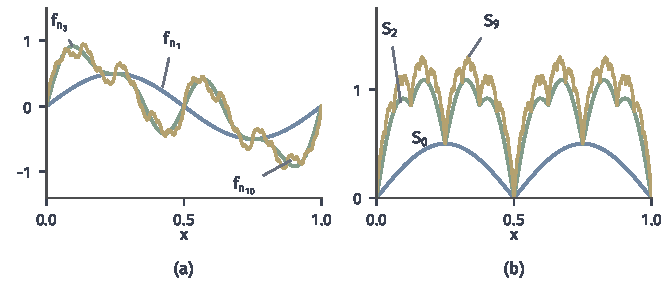
\includegraphics[width=112mm]{figures/04-spaces-measures-and-geometry/03-function-spaces/matplotlib/nspace-fast-subsequence/figure.pdf}
  \caption{完备性证明中的快速子列与控制函数。这里$f_{n_1}(x)=\tfrac12\sin(2\pi x)$，相邻差$f_{n_{k+1}}-f_{n_k}=2^{-k}\sin(2^{k+1}\pi x)$。(a)$f_{n_1},f_{n_3},f_{n_{10}}$，修正项越来越小。(b)控制函数$S_0,S_2,S_9$，随$m$单调上升且有界，每一项$\lvert f_{n_k}\rvert$都不超过它们的极限$S$。}
  \label{fig:nspace-fast-subsequence}
\end{BookInlineFigure}

\begin{theorem}[$L^p$收敛列的几乎处处收敛子列]
\label{thm:nspace-lp-ae-subsequence}
设$1\leq p<\infty$，在$L^p(\mu)$中$f_n\to f$。则存在子列$(f_{n_k})$，使$f_{n_k}\to f$几乎处处成立。
\end{theorem}

\begin{proof}
收敛列是柯西列。定理~\ref{thm:nspace-lp-complete}证明的前四步给出子列与函数$\tilde f$，使$f_{n_k}\to\tilde f$几乎处处且在$L^p$中成立。$L^p$中的极限唯一，所以$\tilde f=f$几乎处处，于是$f_{n_k}\to f$几乎处处。
\end{proof}

回到上一节的折线列$(g_n)$，把证明的步骤走一遍。在$L^1[0,1]$中，阶跃函数的等价类$\mathbf 1_{(1/2,1]}$是合法的元素。由式~\eqref{eq:nspace-ramp-distance}，取$n_k=2^k$时相邻误差为
\[
 \lVert g_{2^{k+1}}-g_{2^k}\rVert_1=\frac1{2^{k+1}}-\frac1{2^{k+2}}=2^{-k-2},
\]
对$k\geq1$求和得$\tfrac14$。

$g_n$关于$n$单调不减，所以控制函数中的绝对值可以去掉，并逐项相消：
\[
 S_m=g_2+\sum_{k=1}^m\bigl(g_{2^{k+1}}-g_{2^k}\bigr)=g_{2^{m+1}}.
\]
令$m\to\infty$，得到$S=\mathbf 1_{(1/2,1]}$，这正是候选极限。它的范数$\lVert S\rVert_1=\tfrac12$，恰好等于证明中的上界$C=\lVert g_2\rVert_1+\tfrac14=\tfrac14+\tfrac14$。

最后计算依范数的误差。折线与阶跃函数只在一个底为$\tfrac1n$、高为$1$的三角形上不同，所以
\[
 \lVert g_n-\mathbf 1_{(1/2,1]}\rVert_1=\frac1{2n}\to0.
\]
在$L^1$中折线列有了极限。阶跃函数在$\tfrac12$处取什么值无关紧要，这正是取等价类的用意。在计数测度下，定理~\ref{thm:nspace-lp-complete}说明每个$\ell^p$（$1\leq p<\infty$）都是Banach空间。

\section{\texorpdfstring{$L^\infty$}{L-infinity}空间}
\label{sec:nspace-linfty-space}

图~\ref{fig:nspace-lp-weight}显示，$p$越大，$L^p$范数越看重大偏差，$p\to\infty$时只剩下最大偏差。向量的情形正是这样：$\lVert v\rVert_p\to\max_i\lvert v_i\rvert$。但等价类中的代表可以在零测集上任意改值，普通的上确界会被单个点左右，对等价类没有确定的意义。本节建立只看“几乎处处”的上界，得到$L^\infty$空间。本节仍固定测度空间$(X,\mathcal A,\mu)$。

\paragraph{本质上确界}
普通上确界要求$\lvert f(x)\rvert\leq M$在每一点都成立；对等价类而言，合理的要求是在某个零测集之外成立。

\begin{definition}[本质上确界与$L^\infty$]
\label{def:nspace-linfty}
对可测函数$f$，定义
\begin{equation}
 \lVert f\rVert_\infty=\inf\{M\geq0:\ \mu(\{x:\lvert f(x)\rvert>M\})=0\},
 \label{eq:nspace-esssup}
\end{equation}
称为$\lvert f\rvert$的\term{本质上确界}（essential supremum），约定空集的下确界为$+\infty$。本质上确界有限的可测函数称为\term{本质有界}（essentially bounded）的，其几乎处处等价类全体记为$L^\infty(\mu)$。
\end{definition}

先看下确界能否取到。设$M_0=\lVert f\rVert_\infty<\infty$。对每个正整数$k$，$M_0+1/k$大于下确界，所以$\{\lvert f\rvert>M_0+1/k\}$是零测集。它们的并
\[
 \{\lvert f\rvert>M_0\}=\bigcup_{k\geq1}\Bigl\{\lvert f\rvert>M_0+\frac1k\Bigr\}
\]
是可数个零测集之并，仍为零测集。所以下确界可以达到：
\begin{equation}
 \lvert f\rvert\leq\lVert f\rVert_\infty\quad\text{几乎处处}.
 \label{eq:nspace-esssup-attained}
\end{equation}
由此也看出数值不依赖代表：若$g\sim_\mu f$，则$\{\lvert g\rvert>M\}\subseteq\{\lvert f\rvert>M\}\cup\{f\neq g\}$，反之亦然，两者的本质上确界相同。

\paragraph{与逐点上确界的比较}
本质上确界与普通上确界可以相差很远。在$[0,1]$上取Lebesgue测度，令$f(x)=x$，再把$f(\tfrac12)$改为$2$。普通上确界是$2$；而$\lvert f\rvert\leq1$只在单点$\{\tfrac12\}$处不成立，单点零测，所以本质上确界是$1$，如图~\ref{fig:nspace-essential-sup}所示。

\begin{BookInlineFigure}
  \centering
  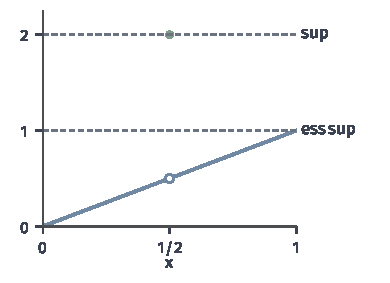
\includegraphics[width=66mm]{figures/04-spaces-measures-and-geometry/03-function-spaces/matplotlib/nspace-essential-sup/figure.pdf}
  \caption{本质上确界忽略零测集。$[0,1]$上取Lebesgue测度，$f(x)=x$，只把$f(\tfrac12)$改为$2$（绿点为改动后的值，空心圈为原值）。普通上确界被这一个点抬到$2$，单点的测度为零，本质上确界仍为$1$。}
  \label{fig:nspace-essential-sup}
\end{BookInlineFigure}

更极端地，有理点的指示函数$\mathbf 1_{\mathbb Q\cap[0,1]}$的普通上确界是$1$，本质上确界是$0$，因为有理点只有可数个，组成零测集。

两者在一个常见情形下一致。若$f$在区间$[a,b]$上连续，对任意$M<\sup\lvert f\rvert$，集合$\{\lvert f\rvert>M\}$是非空的相对开集，含有一个正长度的区间，测度为正，所以本质上确界不小于普通上确界，二者相等。另一方面，$\lVert f\rVert_\infty\leq M$只保证零测集之外$\lvert f\rvert\leq M$，并不保证类中任意一个代表在每一点都受这个界控制。

取$\mathbb N_+$上的计数测度，只有空集零测，本质上确界就是普通上确界，得到有界数列空间
\begin{equation}
 \ell^\infty=\Bigl\{x:\ \sup_{k}\lvert x_k\rvert<\infty\Bigr\},\qquad \lVert x\rVert_\infty=\sup_k\lvert x_k\rvert.
 \label{eq:nspace-ellinfty}
\end{equation}
常数列$(1,1,\ldots)$属于$\ell^\infty$，却不属于任何$\ell^p$（$p<\infty$）。第~\ref{chap:functions-as-vectors}章用$\ell^\infty$中两两距离为$1$的不可数个$0$--$1$数列，说明了它没有可数的级数表示。

\paragraph{范数公理}
$\lVert\cdot\rVert_\infty$在$L^\infty(\mu)$上是范数，论证的关键是把例外集合合并成一个零测集。

正定性：若$\lVert f\rVert_\infty=0$，由式~\eqref{eq:nspace-esssup-attained}，$\lvert f\rvert\leq0$几乎处处，即$[f]$是零元素。齐次性：$c\neq0$时，
\[
 \{\lvert cf\rvert>\lvert c\rvert M\}=\{\lvert f\rvert>M\},
\]
对$M$取下确界即得；$c=0$时两边都是零。

三角不等式：$\lvert f\rvert\leq\lVert f\rVert_\infty$在零测集$N_f$之外成立，$\lvert g\rvert\leq\lVert g\rVert_\infty$在零测集$N_g$之外成立。于是在$N_f\cup N_g$之外，
\[
 \lvert f+g\rvert\leq\lvert f\rvert+\lvert g\rvert\leq\lVert f\rVert_\infty+\lVert g\rVert_\infty.
\]
例外集仍是零测集，所以右边是$\lvert f+g\rvert$的一个本质上界，三角不等式成立。这同时说明$L^\infty(\mu)$对加法封闭。

\paragraph{\texorpdfstring{$L^1$}{L1}与\texorpdfstring{$L^\infty$}{L-infinity}的Hölder估计}
Hölder不等式要求$1<p<\infty$。在端点处，$p=1$的共轭指数应当是$q=\infty$，相应的估计是：若$f\in L^1(\mu)$、$g\in L^\infty(\mu)$，则
\begin{equation}
 \int_X\lvert fg\rvert\,d\mu\leq\lVert f\rVert_1\,\lVert g\rVert_\infty .
 \label{eq:nspace-holder-endpoint}
\end{equation}

证明只需一步。由式~\eqref{eq:nspace-esssup-attained}，几乎处处有
\[
 \lvert fg\rvert\leq\lvert f\rvert\,\lVert g\rVert_\infty,
\]
两边积分即可。约定$1/\infty=0$后，Hölder不等式对所有满足$\tfrac1p+\tfrac1q=1$的$1\leq p,q\leq\infty$都成立。

这个估计说明，固定$g\in L^\infty$，$f\mapsto\int fg\,d\mu$是$L^1$上的线性读取，其大小受$\lVert g\rVert_\infty\lVert f\rVert_1$控制。第~\ref{chap:linear-functionals}章将从这样的配对出发研究$L^p$上的线性泛函。

\paragraph{完备性}
$L^\infty$的完备性与$L^p$（$p<\infty$）的证明方式不同。这里没有积分可以累计，却可以把可数个例外集合并成一个零测集，在它的补集上回到一致收敛的论证。

\begin{theorem}[$L^\infty$的完备性]
\label{thm:nspace-linfty-complete}
对任意测度空间，$L^\infty(\mu)$是Banach空间。
\end{theorem}

\begin{proof}
设$(f_n)$是$L^\infty(\mu)$中的柯西列，取定各项的可测代表。对每一对$m,n$，由式~\eqref{eq:nspace-esssup-attained}，在某个零测集$E_{m,n}$之外有
\[
 \lvert f_n-f_m\rvert\leq\lVert f_n-f_m\rVert_\infty.
\]
令$E=\bigcup_{m,n}E_{m,n}$，它是可数个零测集之并，仍为零测集。

在$X\setminus E$上，所有这些不等式同时成立。给定$\varepsilon>0$，取$N$使$m,n\geq N$时$\lVert f_n-f_m\rVert_\infty<\varepsilon$，则
\[
 \sup_{x\notin E}\lvert f_n(x)-f_m(x)\rvert\leq\varepsilon,\qquad m,n\geq N,
\]
即$(f_n)$在$X\setminus E$上一致柯西。$\mathbb K$完备，所以$f_n$在$X\setminus E$上一致收敛到某个函数$f$；在$E$上令$f=0$。$f$是可测函数列在$X\setminus E$上的逐点极限，因而可测。

在上式中令$m\to\infty$，得到$n\geq N$时
\[
 \sup_{x\notin E}\lvert f_n(x)-f(x)\rvert\leq\varepsilon.
\]
$E$零测，所以$\lVert f_n-f\rVert_\infty\leq\varepsilon$，即$f_n\to f$依范数成立。最后，取$n_0\geq N$，由三角不等式，
\[
 \lVert f\rVert_\infty\leq\lVert f_{n_0}\rVert_\infty+\varepsilon<\infty,
\]
所以$f\in L^\infty(\mu)$。
\end{proof}

两种完备性证明可以对照着看。有限$p$的论证没有一致性可用，只能先抽子列得到几乎处处收敛，再用Fatou引理把逐点信息转为积分信息。$p=\infty$的论证则把可数个例外集合并成一个零测集，在补集上做一致收敛，与连续函数空间的论证相同，只是“处处”换成了“零测集之外”。

在计数测度下，这个定理说明$\ell^\infty$是Banach空间。

\section{函数列的收敛}
\label{sec:nspace-convergence-of-sequences}

有了具体的赋范函数空间，同一列函数就可以在几种意义下讨论收敛：每个输入处的值是否收敛，所有输入上的最大误差是否趋于零，积分误差是否趋于零，误差超过给定阈值的区域是否越来越小。把函数看作向量时，它们分别对应“逐分量”“最大分量”“加权和”和“超差分量的份额”。

有限维向量的这几种收敛等价，函数列的收敛方式之间却只有在附加条件下才能互相推出。第~\ref{chap:integration}章已经用逐点与几乎处处收敛建立了单调收敛和支配收敛定理，本节把这些收敛方式放在一起比较，并用一致可积性补上从依测度收敛到$L^1$收敛所需的条件。

本节固定测度空间$(X,\mathcal A,\mu)$与一列可测函数$f_n$及可测函数$f$，它们几乎处处取有限值。

\subsection{逐点、一致与\texorpdfstring{$L^p$}{Lp}收敛}
\label{sec:nspace-pointwise-uniform-lp}

逐点收敛与一致收敛是对函数本身的要求，第~\ref{chap:metric-space-maps}章已经定义：逐点收敛允许达到给定精度所需的序号依赖于$x$，一致收敛要求同一个序号对所有$x$有效。$L^p$收敛（$1\leq p<\infty$）则是$\lVert f_n-f\rVert_p\to0$，它只看误差$p$次幂的积分。

\paragraph{代表的选择}
这三种收敛对零测集的态度不同。逐点收敛和一致收敛是对选定的代表说的：把$f_n$在一个零测集上改值，可能破坏逐点收敛，也可能把一致收敛的序列变得不一致收敛。

所以在等价类上讨论时，应当改用两个说法。一是几乎处处收敛，即存在零测集$E$使$f_n(x)\to f(x)$对$x\notin E$成立；二是本质一致收敛，即$\lVert f_n-f\rVert_\infty\to0$。

$L^p$收敛和下一小节的依测度收敛只依赖等价类：改动零测集上的值不改变任何积分，也不改变任何集合的测度。

\paragraph{一致收敛推出\texorpdfstring{$L^p$}{Lp}收敛的条件}
一致收敛控制所有点上的误差，积分误差自然也受控制，但这需要总测度有限。若$\mu(X)<\infty$，由$\lvert f_n-f\rvert\leq\lVert f_n-f\rVert_\infty$几乎处处成立，取$p$次幂后积分，得到
\begin{equation}
 \lVert f_n-f\rVert_p\leq\mu(X)^{1/p}\,\lVert f_n-f\rVert_\infty ,
 \label{eq:nspace-uniform-to-lp}
\end{equation}
所以本质一致收敛推出每个$L^p$收敛。测度无限时这一推论失败。在$\mathbb R$上取Lebesgue测度与$h_n=\tfrac1n\mathbf 1_{[0,n]}$，则
\[
 \lVert h_n\rVert_\infty=\frac1n\to0,\qquad \lVert h_n\rVert_1=1.
\]
高度在降低，支撑却在扩大，总面积不变。

不同指数之间也有类似的比较，同样依赖有限测度。设$\mu(X)<\infty$，$1\leq p<r<\infty$。对$\lvert h\rvert^p\cdot1$用Hölder不等式，指数取$r/p$及其共轭指数$r/(r-p)$，得到
\[
 \int_X\lvert h\rvert^p\,d\mu\leq\Bigl(\int_X\lvert h\rvert^r\,d\mu\Bigr)^{p/r}\mu(X)^{1-p/r}.
\]
两边开$p$次方，整理成
\begin{equation}
 \lVert h\rVert_p\leq\mu(X)^{1/p-1/r}\lVert h\rVert_r.
 \label{eq:nspace-lp-inclusion}
\end{equation}
取$h=f_n-f$，$L^r$收敛推出$L^p$收敛。把式~\eqref{eq:nspace-lp-inclusion}看作包含映射$L^r\to L^p$的有界性，是第~\ref{chap:linear-operators}章的内容。

\paragraph{三个对照序列}
图~\ref{fig:nspace-convergence-modes}与表~\ref{tab:nspace-convergence-modes}对照了$[0,1]$上Lebesgue测度下的三个序列，它们标出了各收敛方式之间不能互推的边界。

\begin{BookInlineFigure}
  \centering
  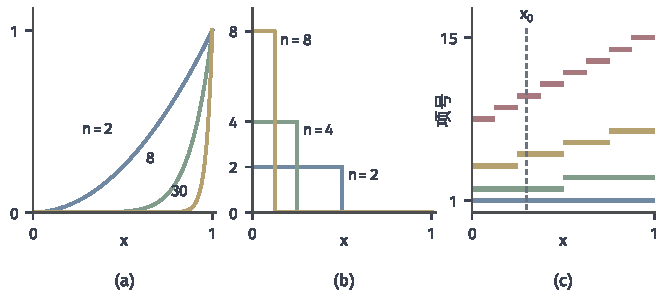
\includegraphics[width=112mm]{figures/04-spaces-measures-and-geometry/03-function-spaces/matplotlib/nspace-convergence-modes/figure.pdf}
  \caption{三种收敛方式的反例。(a)$x^n$，$n=2,8,30$：除$x=1$外逐点趋于$0$，$L^p$范数趋于零，最大误差恒为$1$。(b)窄尖峰$n\mathbf 1_{(0,1/n)}$，$n=2,4,8$：每一点最终为零，积分恒为$1$。(c)打字机序列的前$15$项，第$k$层（$k=0,1,2,3$，蓝、绿、黄、红）把$[0,1)$等分为$2^k$段；纵轴为项号，横条为支撑，竖虚线$x=x_0$在每一层恰好穿过一个横条。}
  \label{fig:nspace-convergence-modes}
\end{BookInlineFigure}

\begin{BookInlineTable}
  \centering
  \begin{tabular}{@{}lccc@{}}
    \toprule
    序列 & 逐点收敛到$0$ & $L^1$收敛到$0$ & 一致收敛到$0$ \\
    \midrule
    $x^n$ & 除$x=1$外 & 是 & 否 \\
    $n\mathbf 1_{(0,1/n)}$ & 是（处处） & 否 & 否 \\
    打字机序列 & 处处不收敛 & 是 & 否 \\
    \bottomrule
  \end{tabular}
  \caption{$[0,1]$上Lebesgue测度下三个序列的收敛性质。}
  \label{tab:nspace-convergence-modes}
\end{BookInlineTable}

先看$x^n$。它的$L^p$范数为
\[
 \lVert x^n\rVert_p=(np+1)^{-1/p}\to0.
\]
逐点极限在$x=1$处为$1$、其余处为$0$。单点零测，所以作为$L^p$中的元素，逐点极限与零元素相同，两种说法并不矛盾。最大误差恒为$1$，不一致收敛。

再看窄尖峰$g_n=n\mathbf 1_{(0,1/n)}$。对$x>0$，只要$n>1/x$就有$g_n(x)=0$，所以处处收敛到$0$。但积分的值不变：
\[
 \lVert g_n\rVert_1=n\cdot\frac1n=1.
\]
逐点收敛允许不同位置在不同时刻进入误差带，因而管不住越来越窄、越来越高的峰。即使总测度有限，逐点收敛也推不出$L^p$收敛。

\begin{example}[打字机序列]
\label{ex:nspace-typewriter}
对$k=0,1,2,\ldots$与$j=0,\ldots,2^k-1$，令
\[
 h_{k,j}=\mathbf 1_{[j2^{-k},(j+1)2^{-k})},
\]
按$k$从小到大、同一层内按$j$从小到大排成一列$h_{0,0},h_{1,0},h_{1,1},h_{2,0},\ldots$。第$k$层每一项的范数为
\[
 \lVert h_{k,j}\rVert_p=2^{-k/p},
\]
随项号增大趋于零，所以序列在每个$L^p$（$p<\infty$）中收敛到$0$。

但对每个$x_0\in[0,1)$，每一层恰好有一项在$x_0$处取$1$，其余项取$0$。所以数列$(h_{k,j}(x_0))$中$0$和$1$都出现无穷多次，在任何一点都不收敛。$L^p$收敛推不出逐点收敛，也推不出几乎处处收敛。
\end{example}

打字机序列虽然整列不逐点收敛，定理~\ref{thm:nspace-lp-ae-subsequence}却保证它有几乎处处收敛的子列。这里可以直接写出一个：子列$h_{k,0}=\mathbf 1_{[0,2^{-k})}$对每个$x>0$在$2^{-k}<x$后恒为零，所以在$(0,1]$上逐点收敛到$0$，例外只有零测点$x=0$。

\subsection{依测度收敛}
\label{sec:nspace-convergence-in-measure}

逐点收敛逐个检查位置，$L^p$收敛累计误差的大小。还有一种更粗的要求：不管误差具体多大，只问误差超过某个阈值的区域有多大。用向量的语言说，它只看超差分量所占的份额。

\begin{definition}[依测度收敛]
\label{def:nspace-convergence-in-measure}
若对每个$\varepsilon>0$，
\begin{equation}
 \lim_{n\to\infty}\mu\bigl(\{x:\lvert f_n(x)-f(x)\rvert>\varepsilon\}\bigr)=0,
 \label{eq:nspace-convergence-in-measure}
\end{equation}
称$f_n$\term{依测度收敛}（convergence in measure）到$f$。
\end{definition}

定义只控制“大误差出现的范围”，不管大误差有多大，也不管它出现在哪里。窄尖峰$n\mathbf 1_{(0,1/n)}$依测度收敛到$0$：对任意$\varepsilon>0$，超差集合至多是$(0,1/n)$，测度$1/n\to0$。它的$L^1$误差却恒为$1$，所以依测度收敛推不出$L^1$收敛。打字机序列的第$k$层超差集合是一个长为$2^{-k}$的区间，同样依测度收敛到$0$，而它处处不逐点收敛。

\paragraph{\texorpdfstring{$L^p$}{Lp}收敛推出依测度收敛}
积分误差小，大误差所占的区域就小。对$1\leq p<\infty$与$\varepsilon>0$，在超差集合$A_n=\{\lvert f_n-f\rvert>\varepsilon\}$上有$\lvert f_n-f\rvert^p>\varepsilon^p$，所以
\begin{equation}
 \varepsilon^p\mu(A_n)\leq\int_{A_n}\lvert f_n-f\rvert^p\,d\mu\leq\lVert f_n-f\rVert_p^p .
 \label{eq:nspace-chebyshev}
\end{equation}
这是\term{Chebyshev不等式}（Chebyshev inequality）。若$\lVert f_n-f\rVert_p\to0$，则$\mu(A_n)\to0$，即依测度收敛。这一推论不要求测度有限。

取$p=1$，用$[0,1]$上的三角形$h(x)=1-\lvert2x-1\rvert$走一遍，$\varepsilon=\tfrac12$。超差集合是$A=(\tfrac14,\tfrac34)$，$\mu(A)=\tfrac12$，式~\eqref{eq:nspace-chebyshev}的两边是
\[
 \varepsilon\,\mu(A)=\frac14,\qquad \lVert h\rVert_1=\frac12.
\]
图~\ref{fig:nspace-chebyshev}显示了这个不等式的来源：高为$\varepsilon$、宽为$\mu(A)$的矩形完全落在曲线下方。

\begin{BookInlineFigure}
  \centering
  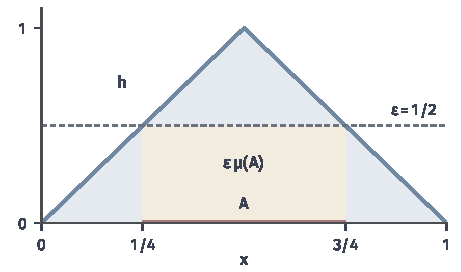
\includegraphics[width=78mm]{figures/04-spaces-measures-and-geometry/03-function-spaces/matplotlib/nspace-chebyshev/figure.pdf}
  \caption{Chebyshev不等式，取$h(x)=1-\lvert2x-1\rvert$、$\varepsilon=\tfrac12$。红线是超差集合$A=(\tfrac14,\tfrac34)$，黄色矩形面积$\varepsilon\,\mu(A)=\tfrac14$，含于面积为$\lVert h\rVert_1=\tfrac12$的蓝色区域之内。}
  \label{fig:nspace-chebyshev}
\end{BookInlineFigure}

\paragraph{有限测度下几乎处处收敛推出依测度收敛}
几乎处处收敛说每一点（零测集之外）迟早进入误差带，依测度收敛说没进入误差带的区域在缩小。在有限测度空间中，前者推出后者。

\begin{theorem}[几乎处处收敛推出依测度收敛]
\label{thm:nspace-ae-to-measure}
设$\mu(X)<\infty$，$f_n\to f$几乎处处。则$f_n$依测度收敛到$f$。
\end{theorem}

\begin{proof}
固定$\varepsilon>0$，令
\[
 B_N=\bigcup_{n\geq N}\{\lvert f_n-f\rvert>\varepsilon\},
\]
它随$N$单调下降。若$x\in\bigcap_NB_N$，则有无穷多个$n$使$\lvert f_n(x)-f(x)\rvert>\varepsilon$，$f_n(x)$不收敛到$f(x)$。所以$\bigcap_NB_N$含于不收敛点的集合，是零测集。

$\mu(B_1)\leq\mu(X)<\infty$，由测度的上连续性，
\[
 \mu(B_N)\to\mu\Bigl(\bigcap_NB_N\Bigr)=0.
\]
而$\{\lvert f_N-f\rvert>\varepsilon\}\subseteq B_N$，所以它的测度也趋于零。
\end{proof}

上连续性要求$\mu(B_1)<\infty$，有限测度正是用在这里。测度无限时结论失败：在$\mathbb R$上取Lebesgue测度与$f_n=\mathbf 1_{[n,n+1]}$，每一点在$n>x$后都有$f_n(x)=0$，处处收敛到$0$；但$\mu(\{f_n>\tfrac12\})=1$，不依测度收敛。

\paragraph{依测度收敛列的几乎处处收敛子列}
依测度收敛推不出几乎处处收敛，打字机序列就是例子。但和$L^p$收敛一样，总可以抽出一个几乎处处收敛的子列。

\begin{theorem}[依测度收敛的子列]
\label{thm:nspace-measure-subsequence}
设$f_n$依测度收敛到$f$。则存在子列$(f_{n_k})$，使$f_{n_k}\to f$几乎处处。
\end{theorem}

\begin{proof}
由定义，可以递归地取$n_1<n_2<\cdots$，使$E_k=\{\lvert f_{n_k}-f\rvert>2^{-k}\}$满足$\mu(E_k)<2^{-k}$。令$F_j=\bigcup_{k\geq j}E_k$，则
\[
 \mu(F_j)\leq\sum_{k\geq j}2^{-k}=2^{1-j}.
\]
若$x\notin F_j$，则对所有$k\geq j$有$\lvert f_{n_k}(x)-f(x)\rvert\leq2^{-k}$，所以$f_{n_k}(x)\to f(x)$。

于是不收敛的点都落在$\bigcap_jF_j$中，而$\mu(\bigcap_jF_j)\leq\mu(F_j)\leq2^{1-j}$对每个$j$成立，这个集合是零测集。
\end{proof}

证明的想法是挑选超差集合测度可求和的子列，使“无穷多次超差”的点只能组成零测集。这里没有用到测度有限。结合Chebyshev不等式，它也给出了定理~\ref{thm:nspace-lp-ae-subsequence}的另一个证明。

\subsection{一致可积性}
\label{sec:nspace-uniform-integrability}

窄尖峰依测度收敛到$0$，$L^1$误差却恒为$1$：峰越来越窄，但越来越高，积分始终集中在测度趋零的区域上。要从依测度收敛得到$L^1$收敛，需要防止积分躲进小区域里的大取值中。第~\ref{chap:integration}章的支配收敛定理用一个共同的可积上界做到这一点；一致可积性是更弱、却恰好够用的条件。本小节设$\mu(X)<\infty$。

\begin{definition}[一致可积]
\label{def:nspace-uniform-integrability}
设$\mu(X)<\infty$，$\{f_n\}\subseteq L^1(\mu)$。若
\begin{equation}
 \lim_{M\to\infty}\ \sup_{n}\int_{\{\lvert f_n\rvert>M\}}\lvert f_n\rvert\,d\mu=0,
 \label{eq:nspace-uniform-integrability}
\end{equation}
称$\{f_n\}$\term{一致可积}（uniformly integrable）。
\end{definition}

对单个可积函数$f$，总有
\[
 \int_{\{\lvert f\rvert>M\}}\lvert f\rvert\,d\mu\to0\qquad(M\to\infty).
\]
这是因为被积函数$\lvert f\rvert\mathbf 1_{\{\lvert f\rvert>M\}}$被$\lvert f\rvert$控制，且在$\lvert f\rvert<\infty$的点处当$M\to\infty$时趋于零，由支配收敛定理即得。一致可积要求这件事对整族函数以同样的速度发生，即大取值区域上的积分一致地小。

\paragraph{尖峰与共同上界}
窄尖峰不是一致可积的。对任意$M$，当$n>M$时$\{g_n>M\}=(0,1/n)$，其上的积分为$1$，所以
\[
 \sup_n\int_{\{g_n>M\}}g_n\,d\mu=1
\]
不随$M$趋于零。这正是它不$L^1$收敛的原因。

把峰的高度从$n$压到$\sqrt n$，情况就变了。令$f_n=\sqrt n\,\mathbf 1_{(0,1/n)}$，只有$\sqrt n>M$时$\{f_n>M\}$才非空，其上的积分为
\[
 \int_{\{f_n>M\}}f_n\,d\mu=\sqrt n\cdot\frac1n=\frac1{\sqrt n}<\frac1M.
\]
上确界不超过$1/M$，所以这一族一致可积。图~\ref{fig:nspace-uniform-integrability}并排画出这两族函数。

\begin{BookInlineFigure}
  \centering
  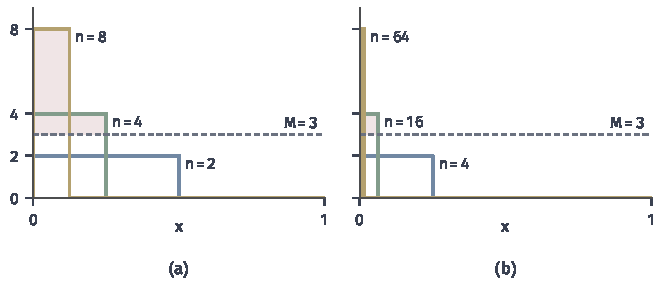
\includegraphics[width=112mm]{figures/04-spaces-measures-and-geometry/03-function-spaces/matplotlib/nspace-uniform-integrability/figure.pdf}
  \caption{尖峰的一致可积性，阈值$M=3$，浅红色为函数高于$M$的部分。(a)$g_n=n\mathbf 1_{(0,1/n)}$，$n=2,4,8$：每个高于阈值的尖峰，整根矩形的面积都是$1$，阈值抬高也不变。(b)$f_n=\sqrt n\,\mathbf 1_{(0,1/n)}$，$n=4,16,64$：高度相同的情况下宽度小得多，$\{f_n>M\}$上的积分是$1/\sqrt n$，随$n$变小。}
  \label{fig:nspace-uniform-integrability}
\end{BookInlineFigure}

有共同可积上界的族总是一致可积的。若$\lvert f_n\rvert\leq G$几乎处处对所有$n$成立，$G\in L^1$，则$\{\lvert f_n\rvert>M\}\subseteq\{G>M\}$，
\[
 \sup_n\int_{\{\lvert f_n\rvert>M\}}\lvert f_n\rvert\,d\mu\leq\int_{\{G>M\}}G\,d\mu\to0.
\]
窄尖峰没有这样的上界：$\sup_ng_n(x)$在$x\in[\tfrac1{n+1},\tfrac1n)$上等于$n>\tfrac1x-1$，不可积。

\paragraph{一致的小区域控制}
一致可积的族在小区域上的积分也一致地小，这是下面证明要用的形式。对任意可测集$A$与$M>0$，把$A$分成$\lvert f_n\rvert>M$与$\lvert f_n\rvert\leq M$两部分，得到
\begin{equation}
 \int_A\lvert f_n\rvert\,d\mu\leq\int_{\{\lvert f_n\rvert>M\}}\lvert f_n\rvert\,d\mu+M\mu(A).
 \label{eq:nspace-ui-small-sets}
\end{equation}

给定$\eta>0$，先取$M$使第一项对所有$n$都小于$\eta/2$，再令$\delta=\eta/(2M)$，则$\mu(A)<\delta$时$\sup_n\int_A\lvert f_n\rvert\,d\mu<\eta$。取$A=X$还得到$\sup_n\lVert f_n\rVert_1\leq\eta/2+M\mu(X)<\infty$，一致可积的族在$L^1$中有界。

\paragraph{从依测度收敛到\texorpdfstring{$L^1$}{L1}收敛}
有了小区域上的一致控制与$L^1$有界性，就可以把依测度收敛加强为$L^1$收敛：大误差区域的测度趋于零，一致可积保证这些区域上的积分也趋于零。

\begin{theorem}[依测度收敛与一致可积推出\texorpdfstring{$L^1$}{L1}收敛]
\label{thm:nspace-vitali}
设$\mu(X)<\infty$，$\{f_n\}\subseteq L^1(\mu)$一致可积，且$f_n$依测度收敛到可测函数$f$。则$f\in L^1(\mu)$，且$\lVert f_n-f\rVert_1\to0$。
\end{theorem}

\begin{proof}
先证$f$可积。由定理~\ref{thm:nspace-measure-subsequence}，有子列$f_{n_k}\to f$几乎处处。由Fatou引理与上面的$L^1$有界性，
\[
 \int_X\lvert f\rvert\,d\mu\leq\liminf_{k\to\infty}\int_X\lvert f_{n_k}\rvert\,d\mu\leq\sup_n\lVert f_n\rVert_1<\infty.
\]

再估计误差。给定$\varepsilon>0$与$\eta>0$，令$A_n=\{\lvert f_n-f\rvert>\varepsilon\}$。在$A_n$之外误差不超过$\varepsilon$，在$A_n$上用三角不等式，所以
\[
 \int_X\lvert f_n-f\rvert\,d\mu\leq\varepsilon\,\mu(X)+\int_{A_n}\lvert f_n\rvert\,d\mu+\int_{A_n}\lvert f\rvert\,d\mu.
\]

对族$\{f_n\}$取上一段的$\delta_1$；单个可积函数$f$构成的族$\{f\}$也一致可积，对它取$\delta_2$。依测度收敛给出$N$，使$n\geq N$时$\mu(A_n)<\min(\delta_1,\delta_2)$，此时后两项都小于$\eta$。于是$n\geq N$时
\[
 \lVert f_n-f\rVert_1\leq\varepsilon\,\mu(X)+2\eta.
\]
$\varepsilon,\eta$任意，故$\lVert f_n-f\rVert_1\to0$。
\end{proof}

证明把误差分成两部分：在误差不超过$\varepsilon$的区域上，贡献至多$\varepsilon\mu(X)$；误差超过$\varepsilon$的区域测度趋零，依测度收敛只保证这一点，其上的积分则由一致可积控制。有限测度用在两处：$\varepsilon\mu(X)$有限，以及式~\eqref{eq:nspace-ui-small-sets}给出$L^1$有界。

用前面的例子验证。$f_n=\sqrt n\,\mathbf 1_{(0,1/n)}$一致可积，又依测度收敛到$0$，定理给出$\lVert f_n\rVert_1\to0$；直接计算也得到$\lVert f_n\rVert_1=1/\sqrt n\to0$。窄尖峰不满足一致可积，定理不能用，结论也确实不成立。

\paragraph{回到支配收敛}
若$f_n\to f$几乎处处，且$\lvert f_n\rvert\leq G\in L^1$，则在有限测度下，定理~\ref{thm:nspace-ae-to-measure}给出依测度收敛，上面的论证给出一致可积，于是定理~\ref{thm:nspace-vitali}推出$\lVert f_n-f\rVert_1\to0$。这就回到了第~\ref{chap:integration}章的支配收敛定理。

共同可积上界只是一致可积的充分条件。一致可积只要求大取值区域上的积分一致地小，允许没有共同可积上界的族。

反过来，在有限测度下，$L^1$收敛的序列一定一致可积。证明要把前面的小区域控制转回大取值集合，篇幅较长，读者可查阅测度论的教材。所以在有限测度下，一致可积恰好刻画了依测度收敛何时能升级为$L^1$收敛。

\section{本章小结}
\label{sec:nspace-summary}

章首的问题是：比较两个函数时用哪一种误差，以及误差趋零的过程能否在空间内找到终点。范数回答前一个问题。它满足正定性、齐次性和三角不等式，诱导出距离、收敛和柯西列；最大绝对值看最坏位置，积分看总体累计，两者在$C[0,1]$上只有单向的控制$\lVert f\rVert_1\leq\lVert f\rVert_\infty$。有限维中任意两个范数等价，无限维中则不然：借助第~\ref{chap:functions-as-vectors}章两两远离的单位列和一组代数基，可以在任何无限维赋范空间上造出不等价的范数，$x^n$则在$C[0,1]$上给出具体例子。所以无限维中的收敛必须连同范数一起陈述。

完备性回答后一个问题。Banach空间中每个柯西列都有极限；Banach空间的线性子空间完备当且仅当它是闭集，多项式在最大误差下就不闭。紧集上的连续函数在一致范数下完备，证明依靠一致柯西列的极限与一致极限的连续性；非紧定义域上改用有界连续函数，只需补上极限的有界性。同一个$C[0,1]$在积分范数下不完备，逼近阶跃函数的折线列没有连续的极限。

$L^p$与$L^\infty$为积分误差下的极限提供了去处。它们的元素是几乎处处相等的可测函数组成的等价类，因而一般没有点值；计数测度下得到数列空间$\ell^p$与$\ell^\infty$。$L^p$的三角不等式来自Young、Hölder与Minkowski不等式，完备性的证明先抽相邻误差可求和的子列，再用Fatou引理回到积分。$L^\infty$用本质上确界忽略零测集，Hölder不等式在端点$p=1$、$q=\infty$同样成立，完备性来自把可数个例外集合并成一个零测集后的一致收敛。

各种收敛方式控制的误差不同。一致收敛推出$L^p$收敛需要有限测度；逐点收敛管不住窄尖峰，$L^p$收敛推不出逐点收敛，打字机序列是例子；但$L^p$收敛与依测度收敛的序列都有几乎处处收敛的子列。依测度收敛只控制大误差出现的范围，在有限测度下配合一致可积性才推出$L^1$收敛，共同可积上界是一致可积的充分条件，由此回到支配收敛定理。

本章只在单个空间内比较误差。内积带来的正交结构与最佳逼近在第~\ref{chap:inner-product-spaces}章研究；把一个空间放进另一个空间时误差怎样传递，即包含映射的有界性，在第~\ref{chap:linear-operators}章研究；用简单函数、连续函数逼近$L^p$中的元素，在第~\ref{chap:function-approximation}章研究。

